\begin{figure}
  \centering
  \begin{tabular}{ccc}
    \begin{minipage}{0.330\hsize}
      \centering
      $\pi^-\Sigma^+$ mode
      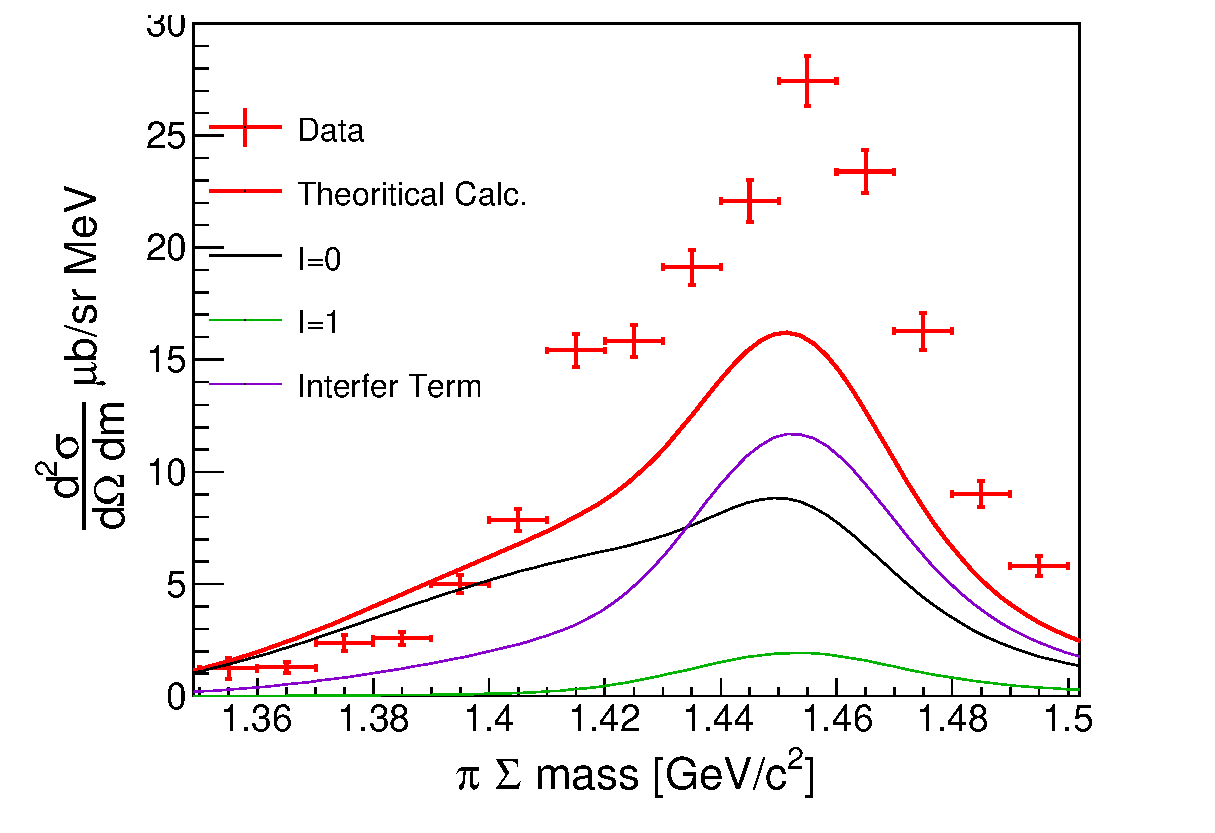
\includegraphics[width=4.5cm]{../pic/Dron/fit_model_B/pimSp_fit.eps}
    \end{minipage}

    \begin{minipage}{0.33\hsize}
      \centering
      $\pi^+\Sigma^-$ mode
      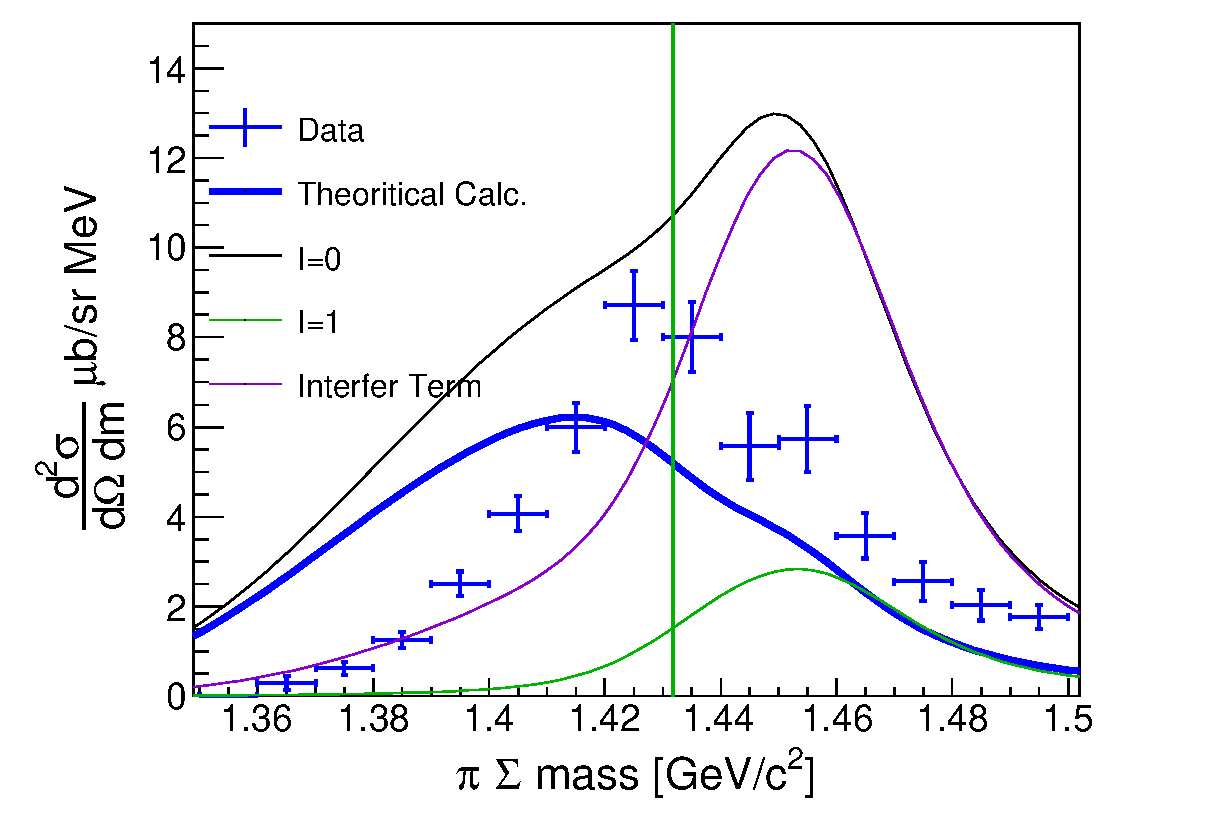
\includegraphics[width=4.5cm]{../pic/Dron/fit_model_B/pipSm_fit.eps}
    \end{minipage}

    \begin{minipage}{0.33\hsize}
      \centering
      $\pi^-\Sigma^0$ mode
      \includegraphics[width=4.5cm]{../pic/Dron/fit_model_B/pimS0_fit.eps}
    \end{minipage}
  \end{tabular}

  \begin{tabular}{cc}
    \begin{minipage}{0.5\hsize}
      \centering
      $I=0$\\
      \includegraphics[width=4.5cm]{../pic/Dron/fit_model_B/I0_fit.eps}
    \end{minipage}
    
    \begin{minipage}{0.5\hsize}
      \centering
      Interfer\\
      \includegraphics[width=4.5cm]{../pic/Dron/fit_model_B/interfer_fit.eps}
    \end{minipage}
  \end{tabular}
  \caption{
    These figures show fitting result about $A_{I=0}$, $A_{I=1}$ and $B$ that is the scaling factor about interference term using model.B
    with same notation of Fig[\ref{fig:fit_A_scale}].
  }
  \label{fig:fit_B}
\end{figure}
